% \lstset{
%     language=C,
%     emph={APPROX, PRECISE, ENDORSE},
%     emphstyle=\bfseries,
%     basicstyle=\ttfamily\small,
%     basewidth=0.53em,
%     aboveskip=1mm plus 1mm minus 1mm,
%     belowskip=1mm plus 1mm minus 1mm,
%     mathescape=true,
%     xleftmargin=\parindent,
% }
% \newcommand{\lil}{\lstinline}

\newcommand{\sysname}{\textsc{Accept}\xspace}
\newcommand{\secref}[1]{Section~\ref{accept:#1}}
\newcommand{\Sref}[1]{\S\ref{accept:#1}}
\newcommand{\plursecref}[1]{\mbox{Sections~{#1}}}
\newcommand{\figref}[1]{Figure~\ref{accept:#1}}
\newcommand{\tabref}[1]{Table~\ref{accept:#1}}
\newcommand{\etal}{et~al.\@\xspace}
\newcommand{\term}[1]{\emph{#1}}
\newcommand{\annpermit}{\lil{ACCEPT_PERMIT}\xspace}
\newcommand{\annforbid}{\lil{ACCEPT_FORBID}\xspace}

% Shifting terminology.
\newcommand{\precisepure}{approximatable\xspace}
\newcommand{\precisepurity}{approximatability\xspace}
\newcommand{\Precisepurity}{Approximatability\xspace}

% Generated results values.
\edef\result#1{%
\ifstrequal{#1}{fft-mlc-cycles}{2.68}{}%
\ifstrequal{#1}{fft-mlc-error}{1\%}{}%
\ifstrequal{#1}{fft-mlc-speedup}{1.13$\times$}{}%
\ifstrequal{#1}{fft-mlc-stripe-cycles}{2.44}{}%
\ifstrequal{#1}{fft-mlc-stripe-error}{4\%}{}%
\ifstrequal{#1}{fft-mlc-stripe-speedup}{1.24$\times$}{}%
\ifstrequal{#1}{image-mlc-cycles}{1.41}{}%
\ifstrequal{#1}{image-mlc-error}{1\%}{}%
\ifstrequal{#1}{image-mlc-flash-cycles}{13.0}{}%
\ifstrequal{#1}{image-mlc-flash-error}{9\%}{}%
\ifstrequal{#1}{image-mlc-flash-speedup}{1.6$\times$}{}%
\ifstrequal{#1}{image-mlc-speedup}{2.14$\times$}{}%
\ifstrequal{#1}{image-mlc-stripe-cycles}{1.41}{}%
\ifstrequal{#1}{image-mlc-stripe-error}{1\%}{}%
\ifstrequal{#1}{image-mlc-stripe-speedup}{2.14$\times$}{}%
\ifstrequal{#1}{jmeint-mlc-cycles}{1.87}{}%
\ifstrequal{#1}{jmeint-mlc-error}{2\%}{}%
\ifstrequal{#1}{jmeint-mlc-speedup}{1.62$\times$}{}%
\ifstrequal{#1}{jmeint-mlc-stripe-cycles}{1.71}{}%
\ifstrequal{#1}{jmeint-mlc-stripe-error}{10\%}{}%
\ifstrequal{#1}{jmeint-mlc-stripe-speedup}{1.77$\times$}{}%
\ifstrequal{#1}{lu-mlc-cycles}{1.98}{}%
\ifstrequal{#1}{lu-mlc-error}{6\%}{}%
\ifstrequal{#1}{lu-mlc-speedup}{1.53$\times$}{}%
\ifstrequal{#1}{lu-mlc-stripe-cycles}{1.98}{}%
\ifstrequal{#1}{lu-mlc-stripe-error}{5\%}{}%
\ifstrequal{#1}{lu-mlc-stripe-speedup}{1.53$\times$}{}%
\ifstrequal{#1}{mc-mlc-cycles}{1.71}{}%
\ifstrequal{#1}{mc-mlc-error}{4\%}{}%
\ifstrequal{#1}{mc-mlc-speedup}{1.77$\times$}{}%
\ifstrequal{#1}{mc-mlc-stripe-cycles}{1.59}{}%
\ifstrequal{#1}{mc-mlc-stripe-error}{10\%}{}%
\ifstrequal{#1}{mc-mlc-stripe-speedup}{1.91$\times$}{}%
\ifstrequal{#1}{ml-mlc-cycles}{1.71}{}%
\ifstrequal{#1}{ml-mlc-error}{6\%}{}%
\ifstrequal{#1}{ml-mlc-flash-cycles}{19.7}{}%
\ifstrequal{#1}{ml-mlc-flash-error}{8\%}{}%
\ifstrequal{#1}{ml-mlc-flash-speedup}{1.05$\times$}{}%
\ifstrequal{#1}{ml-mlc-speedup}{1.77$\times$}{}%
\ifstrequal{#1}{ml-mlc-stripe-cycles}{1.41}{}%
\ifstrequal{#1}{ml-mlc-stripe-error}{0\%}{}%
\ifstrequal{#1}{ml-mlc-stripe-speedup}{2.14$\times$}{}%
\ifstrequal{#1}{mlc-flash-mean-cycles}{16.4}{}%
\ifstrequal{#1}{mlc-flash-mean-speedup}{1.26$\times$}{}%
\ifstrequal{#1}{mlc-mean-cycles}{1.91}{}%
\ifstrequal{#1}{mlc-mean-speedup}{1.59$\times$}{}%
\ifstrequal{#1}{mlc-stripe-mean-cycles}{1.79}{}%
\ifstrequal{#1}{mlc-stripe-mean-speedup}{1.7$\times$}{}%
\ifstrequal{#1}{nn-mlc-cycles}{1.87}{}%
\ifstrequal{#1}{nn-mlc-error}{1\%}{}%
\ifstrequal{#1}{nn-mlc-flash-cycles}{16.5}{}%
\ifstrequal{#1}{nn-mlc-flash-error}{10\%}{}%
\ifstrequal{#1}{nn-mlc-flash-speedup}{1.26$\times$}{}%
\ifstrequal{#1}{nn-mlc-speedup}{1.62$\times$}{}%
\ifstrequal{#1}{nn-mlc-stripe-cycles}{1.71}{}%
\ifstrequal{#1}{nn-mlc-stripe-error}{1\%}{}%
\ifstrequal{#1}{nn-mlc-stripe-speedup}{1.77$\times$}{}%
\ifstrequal{#1}{pa-mlc-cycles}{1.71}{}%
\ifstrequal{#1}{pa-mlc-error}{3\%}{}%
\ifstrequal{#1}{pa-mlc-flash-cycles}{16.5}{}%
\ifstrequal{#1}{pa-mlc-flash-error}{6\%}{}%
\ifstrequal{#1}{pa-mlc-flash-speedup}{1.26$\times$}{}%
\ifstrequal{#1}{pa-mlc-speedup}{1.77$\times$}{}%
\ifstrequal{#1}{pa-mlc-stripe-cycles}{1.59}{}%
\ifstrequal{#1}{pa-mlc-stripe-error}{5\%}{}%
\ifstrequal{#1}{pa-mlc-stripe-speedup}{1.91$\times$}{}%
\ifstrequal{#1}{raytracer-mlc-cycles}{1.59}{}%
\ifstrequal{#1}{raytracer-mlc-error}{7\%}{}%
\ifstrequal{#1}{raytracer-mlc-speedup}{1.91$\times$}{}%
\ifstrequal{#1}{raytracer-mlc-stripe-cycles}{1.59}{}%
\ifstrequal{#1}{raytracer-mlc-stripe-error}{6\%}{}%
\ifstrequal{#1}{raytracer-mlc-stripe-speedup}{1.91$\times$}{}%
\ifstrequal{#1}{recycle-fft-qos-ext}{5\%}{}%
\ifstrequal{#1}{recycle-fft-total-ext}{34\%}{}%
\ifstrequal{#1}{recycle-image-ext}{90\%}{}%
\ifstrequal{#1}{recycle-jmeint-qos-ext}{25\%}{}%
\ifstrequal{#1}{recycle-jmeint-total-ext}{34\%}{}%
\ifstrequal{#1}{recycle-lu-qos-ext}{11\%}{}%
\ifstrequal{#1}{recycle-lu-total-ext}{32\%}{}%
\ifstrequal{#1}{recycle-mc-qos-ext}{32\%}{}%
\ifstrequal{#1}{recycle-mc-total-ext}{34\%}{}%
\ifstrequal{#1}{recycle-mean-all-ext}{23\%}{}%
\ifstrequal{#1}{recycle-mean-nv-ext}{36\%}{}%
\ifstrequal{#1}{recycle-mean-qos-ext}{18\%}{}%
\ifstrequal{#1}{recycle-mean-total-ext}{34\%}{}%
\ifstrequal{#1}{recycle-ml-ext}{17\%}{}%
\ifstrequal{#1}{recycle-nn-ext}{17\%}{}%
\ifstrequal{#1}{recycle-pa-ext}{42\%}{}%
\ifstrequal{#1}{recycle-raytracer-qos-ext}{39\%}{}%
\ifstrequal{#1}{recycle-raytracer-total-ext}{39\%}{}%
\ifstrequal{#1}{recycle-smm-qos-ext}{20\%}{}%
\ifstrequal{#1}{recycle-smm-total-ext}{29\%}{}%
\ifstrequal{#1}{recycle-sor-qos-ext}{20\%}{}%
\ifstrequal{#1}{recycle-sor-total-ext}{32\%}{}%
\ifstrequal{#1}{recycle-zxing-qos-ext}{2\%}{}%
\ifstrequal{#1}{recycle-zxing-total-ext}{37\%}{}%
\ifstrequal{#1}{smm-mlc-cycles}{1.87}{}%
\ifstrequal{#1}{smm-mlc-error}{3\%}{}%
\ifstrequal{#1}{smm-mlc-speedup}{1.62$\times$}{}%
\ifstrequal{#1}{smm-mlc-stripe-cycles}{1.87}{}%
\ifstrequal{#1}{smm-mlc-stripe-error}{2\%}{}%
\ifstrequal{#1}{smm-mlc-stripe-speedup}{1.62$\times$}{}%
\ifstrequal{#1}{sor-mlc-cycles}{2.25}{}%
\ifstrequal{#1}{sor-mlc-error}{3\%}{}%
\ifstrequal{#1}{sor-mlc-speedup}{1.35$\times$}{}%
\ifstrequal{#1}{sor-mlc-stripe-cycles}{2.1}{}%
\ifstrequal{#1}{sor-mlc-stripe-error}{7\%}{}%
\ifstrequal{#1}{sor-mlc-stripe-speedup}{1.44$\times$}{}%
\ifstrequal{#1}{zxing-mlc-cycles}{2.25}{}%
\ifstrequal{#1}{zxing-mlc-error}{4\%}{}%
\ifstrequal{#1}{zxing-mlc-speedup}{1.35$\times$}{}%
\ifstrequal{#1}{zxing-mlc-stripe-cycles}{2.1}{}%
\ifstrequal{#1}{zxing-mlc-stripe-error}{9\%}{}%
\ifstrequal{#1}{zxing-mlc-stripe-speedup}{1.44$\times$}{}%
}


\begin{figure}
\centering
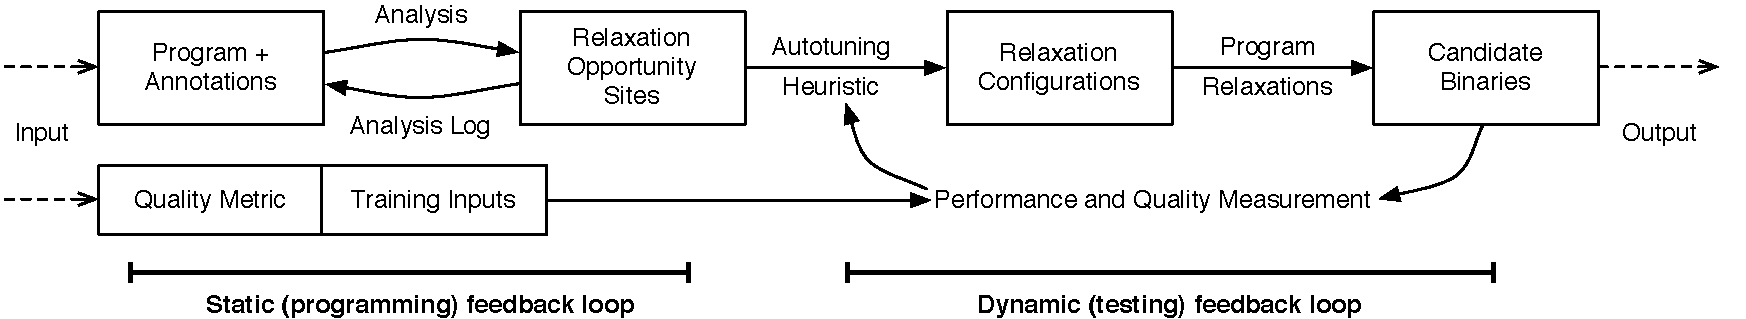
\includegraphics[width=0.9\textwidth]{figs/overview.pdf}
\caption{Overview of the \sysname compiler workflow.}
\label{accept:fig:overview}
\end{figure}

\section{Introduction}\label{sec:intro}

% Energy is an increasingly important consideration for system designers;
% conserving energy enables longer battery life and lower chip temperatures.
%
Recent work on \emph{approximate computing} has exploited the fact that 
many applications, particularly those whose outputs are meant for human
interpretation, can enable more efficient execution at the cost of slightly
inaccurate outputs. 3-D rendering, search, and machine learning
are examples of the many tasks that tolerate inaccuracy.

Research over the past few years has proposed a variety of software and hardware 
approaches to approximate computing, including:
%
producing multiple versions of a program with varying accuracy and choosing
between them at run
time~\cite{green, dynamicknobs};
%
periodically skipping loop iterations~\cite{perforation, qosprof};
%
removing synchronization to reduce contention~\cite{dubstep, quickstep, races-ibm};
%
adjusting floating-point precision~\cite{precimonious};
%
using special low-power hardware
structures that produce wrong results probabilistically~\cite{truffle, flikker};
%
and training hardware neural networks to mimic the behavior of costly
functions~\cite{npu, anpu}.

These proposals share an important distinction
from traditional program optimizations:
they have subtle and broad-ranging effects on safety, reliability, and output
quality.
Some work relies on programmers for manual reasoning to control
these
effects~\cite{npu, flikker, races-ibm, perforation},
while other work proposes automated transformation based on code
patterns or exhaustive search~\cite{green, paraprox, sage}.
Manual code editing can be tedious and error-prone, especially since
important safety invariants are at stake.
Conversely, full automation eliminates a crucial element of
visibility and control.
Programmers must trust the automated system; they have no recourse when
opportunities are missed or invariants are broken.

We propose \sysname
\ifnum\cameraready=1
(an Approximate C Compiler for Energy and Performance Trade-offs),
\else
(a Scalable-Precision Optimizing Compiler Kit),
\fi
a framework for approximation that balances automation with programmer
guidance.
\sysname is \emph{controlled} because it preserves programmer intention
expressed via code annotations.
A static analysis rules out
unintended side effects. The programmer participates in a feedback loop with
the analysis to enable more approximation
opportunities.
\sysname is \emph{practical} because it facilitates a range
of approximation techniques that work on currently available hardware.
Just as a traditional compiler framework provides common tools to support
optimizations,
\sysname's building blocks help implement automatic
approximate transformations based on programmer guidance and dynamic feedback.

\sysname's architecture combines static and dynamic components.
The frontend, built atop LLVM~\cite{llvm}, extends the syntax of C and C++ to
incorporate an \lil{APPROX} keyword that programmers use to annotate types as
in other work~\cite{enerj}.
\sysname's central analysis, \emph{\precisepurity}, identifies coarse-grained
regions of code that can
affect only approximate values.
Coarse region selection is crucial for safe approximation strategies:
client optimizations use the results to
transform code and offload to accelerators while preserving static safety
properties.
After compilation, an autotuning component measures program executions
and uses heuristics to identify program variants that maximize performance and output quality.
To incorporate application insight, \sysname furnishes programmers with feedback
to guide them toward better annotations.


\paragraph{Contributions.}
\sysname is an end-to-end framework that makes existing proposals for approximate
program transformations practical and disciplined.
Its contributions are:
\begin{itemize}
\item A programming model for program relaxation that combines lightweight
annotations with compiler analysis feedback
to guide programmers toward effective relaxations;

\item An autotuning system that efficiently searches for a program's
best approximation parameters;

\item A core analysis library that identifies code that can be safely relaxed
or offloaded to an approximate accelerator;

\item A prototype implementation demonstrating both pure-software optimizations
and hardware acceleration using an off-the-shelf FPGA part.
\end{itemize}

\noindent
We evaluate \sysname across three platforms:
a standard Intel-based server;
a mobile SoC with an on-chip FPGA, which we use as an approximate accelerator;
and an ultra-low-power, energy-harvesting embedded microcontroller where
performance is critical to applications' viability.
The experiments demonstrate average speedups of \result{speedup-x86-mean},
\result{speedup-zynq-mean}, and \result{speedup-msp430-mean} on the
three platforms, respectively,
with quality loss under 10\%.

We also report qualitatively on the programming experience.
Novice C++ programmers were able to apply \sysname to
legacy software to obtain new speedups.
\sysname's combination of static analysis and dynamic measurement alleviates
much of the manual labor from the process of applying
approximation without sacrificing transparency or control.

The \sysname framework is open source and ready for use as research
infrastructure.
It provides the necessary language and compiler support to prototype and
evaluate new strategies for approximation,
reducing the need to reinvent these components for each new research
evaluation.


\section{Overview}

% The primary goal of \sysname is to enable safe, practical, and intuitive
% approximation for general-purpose programs on commodity hardware.  Like previous
% approximation systems~\cite{enerj, relax, flikker}, \sysname involves the programmer in
% application-dependent decisions about where approximation can apply: the
% programmer provides annotations, \sysname highlights opportunities where it can apply program relaxations to improve performance, and possibly offers suggestions to the programmer on code changes that would enable more approximation opportunities. 

To safely and efficiently harness the potential of approximate programs,
\sysname combines three main techniques: (1) a programmer--compiler
feedback loop consisting of source code annotations and an analysis log; (2) a
compiler analysis library
that enables a range of automatic program relaxations; and (3) an autotuning
system that uses dynamic measurements of candidate program relaxations to find
the best balances between efficiency and quality. The final output is a set of
Pareto-optimal versions of the input program that reflect its
efficiency--quality trade-off space.

Figure~\ref{accept:fig:overview} illustrates
how these components make up \sysname's workflow.
Two feedback loops control the impact of
potentially destructive program relaxations: a \emph{static} feedback loop
providing
conservative guarantees
and a complementary \emph{dynamic} feedback loop that measures real
program behavior to choose the best optimizations.
%
A key hypothesis of this work is that neither static nor dynamic constraints
are sufficient, since dynamic measurements cannot offer guarantees and static
constraints do not capture the full complexity of relationships among
relaxations, performance, and output quality. Together, however, the two
feedback loops make \sysname's optimizations both controlled and practical.
%
%\sysname's workflow comprises three main components:

\paragraph{Safety constraints and feedback}
Because program relaxations can have outsized effects on program behavior,
programmers need \emph{visibility} into---and \emph{control} over---the
transformations the compiler applies.
%
To give the programmer fine-grained control over relaxations, \sysname extends
EnerJ's lightweight annotation system (see \chref{enerj}).
%
\sysname gives programmers visibility into the relaxation process via feedback
that identifies which transformations can be applied and which annotations are
constraining it.  Through annotation and feedback, the programmer iterates
toward an annotation set that unlocks new performance benefits while relying on
an assurance that critical computations are unaffected.

\paragraph{Automatic program transformations}
Based on programmer annotations, \sysname's compiler passes apply
transformations that involve only approximate data.
To this end,
\sysname provides a common analysis library that identifies code regions
that can be safely transformed.
We bring \sysname's safety analysis, programmer feedback, and automatic site
identification to existing work
on approximate program transformations~\cite{perforation, races-ibm,
rinard-hotpar, quickstep, dubstep, npu, anpu}.

\paragraph{Autotuning}
While a set of annotations may permit many different safe program relaxations,
not all of them are beneficial.
A practical system must help programmers choose from
among many candidate relaxations for a given program to strike an
optimal balance between performance and quality.
\sysname's autotuner heuristically explores the space of possible relaxed
programs to identify Pareto-optimal variants.



\section{Annotation and Programmer Feedback}
\label{accept:sec:annotation-feedback}

This section describes \sysname's annotations and feedback,
which helps programmers balance safety with approximation.
Rather than proving theoretical accuracy guarantees for restricted programming
models as in other work~\cite{sasa-sas11, zhu-popl12, passert},
\sysname's workflow extends mainstream development practices: it combines
lightweight safety guarantees, programmer insight, and testing to apply
approximation to general code.

\subsection{Annotation Language}
\label{accept:sec:language}

The programmer uses annotations to communicate to the compiler which parts of
a program are safe targets for program relaxation.
\sysname adapts the type system of EnerJ, a language for approximate computing
that was originally developed for bounding the effects of unreliable hardware
components~\cite{enerj}.
As in EnerJ, all types in \sysname are qualified as either \emph{approximate} or
\emph{precise}, with precise being the default.

\paragraph{Information flow and endorsement.}
\sysname's type system uses a standard information-flow
approach to prevent approximate data from affecting precise data.
%
Precise types are strict subtypes of their approximate counterparts, so
variables annotated as approximate cannot be assigned to precise ones without
explicit programmer intervention.  (The opposite direction, wherein precise data
affects approximate data, is permitted.)
%
\sysname's type system is directly derived from EnerJ's~\cite{enerj}, for which
its authors prove a noninterference property ensuring that precise data stays
precise.  The same noninterference guarantee applies to \sysname's
type-qualifier extension for type-safe subsets of C and C++.
Undefined behavior in C and C++ remains undefined in \sysname:
programs that violate type safety can also violate \sysname's guarantees.

Strict information flow can be too constraining.
For example, a program may need to
compute an approximate value, where relaxations can apply, but then check the
resulting output for integrity while treating it as precise:
%
\begin{lstlisting}
APPROX int a = expensiveCall();
cheapChecksumPrecise(a); // illegal
\end{lstlisting}
%
To permit this pattern, \sysname provides an \emph{endorsement} expression
that acts as a cast from an approximate type to its precise equivalent.
The above program fails to typecheck, but using \lil{ENDORSE(a)} as the argument
is legal:
\begin{lstlisting}
APPROX int a = expensiveCall();
cheapChecksumPrecise(ENDORSE(a));
\end{lstlisting}
Endorsements give programmers explicit control over information flow
when dealing with approximate values.

\paragraph{Pointer types.}
For basic, non-reference types, \sysname's dialect of C allows unidirectional
information flow: precise values can be assigned into approximate variables
but not vice-versa. For pointers and references, however,
even precise-to-approximate flow is unsound since
it creates aliases for the same data that disagree on its type.
Pointer types are therefore invariant in the referent type.
The language does not permit approximate pointers---i.e., addresses must be
precise.

\paragraph{Implicit flow.}
Control flow provides an avenue for approximate data to affect precise data
without a direct assignment. For example, \lil{if (a) p = 5;} allows the
variable \lil{a} to affect the value of \lil{p}.
Like EnerJ, \sysname prohibits approximate values from being used in
conditions---specifically, in \lil{if}, \lil{for}, \lil{do}, \lil{while}, and
\lil{switch} statements and in the ternary conditional-expression operator.
Programmers can use endorsements to explicitly circumvent this restriction.

\paragraph{Escape hatches.}
\sysname decides whether program relaxations are safe based on the
\emph{effects} of the statements involved. Section~\ref{accept:sec:relaxations} goes
into more detail, but at a high level, code can be relaxed if its externally
visible effects are approximate.  For example, if \lil{a} is a pointer to
an \lil{APPROX int}, then the statement \lil{*a = 5;} has an approximate effect
on the heap.
Escape hatches from this sound reasoning are critical in a practical
system that must handle legacy code.
To enable or disable specific optimizations, the programmer can
override the compiler's decision about a statement's effects using two
annotations. The \annpermit annotation forces a statement to
be considered approximate
and \annforbid forces it to be precise, forbidding
any relaxations involving it.

These two annotations represent escape hatches from \sysname's normal
reasoning and thus violate the safety guarantees it normally provides.
%
Qualitatively, when annotating programs, we use these
annotations much less frequently than the primary annotations
\lil{APPROX} and \lil{ENDORSE}. We find \annpermit to be
useful when experimentally exploring program behavior before annotating and in
system programming involving memory-mapped registers.  Conversely,
\annforbid is useful for marking parts of the program involved in
introspection. Section~\ref{accept:sec:casestudy} gives more detail on these
experiences.

\subsection{Programmer Feedback}
\label{accept:sec:feedback}

\sysname takes inspiration from parallelizing compilers that use a development
feedback loop to help guide the programmer toward parallelization
opportunities~\cite{canal, deditor}.
It provides
feedback through an \term{analysis log} that describes the relaxations that it
attempted to apply. For example, for \sysname's synchronization-elision
relaxation, the log lists every lexically scoped lock acquire/release pair in
the program. For each relaxation opportunity, it reports whether the relaxation
is safe---whether it involves only approximate data---and, if it is
not, identifies the statements that prevent the relaxation from applying.
We call these statements with
externally visible precise effects \emph{blockers}.

\sysname reports blockers for each failed
relaxation-opportunity site. For example, during the annotation of one program
in our evaluation, \sysname examined this loop:
%
\begin{lstlisting}[numbers=left,firstnumber=650,numbersep=-1pt,numberstyle=\sffamily]
  double myhiz = 0;
  for (long kk=k1; kk<k2; kk++) {
    myhiz += dist(points->p[kk], points->p[0],
      ptDimension) * points->p[kk].weight;
  }
\end{lstlisting}
%
The store to the precise (by default) variable \lil{myhiz}
prevents the loop from being approximable. The analysis log reports:
%
\begin{lstlisting}
loop at streamcluster.cpp:651
blockers: 1
 * streamcluster.cpp:652: store to myhiz
\end{lstlisting}
%
Examining that loop in context, we found that \lil{myhiz} was a weight
accumulator that had little impact on the algorithm, so we changed its type from
\lil{double} to \lil{APPROX double}. On its next execution, \sysname logged the
following message about the same loop, highlighting a new relaxation
opportunity:
%
\begin{lstlisting}
loop at streamcluster.cpp:651
can perforate loop
\end{lstlisting}
%
The feedback loop between the programmer's annotations and the compiler's
analysis log strikes a balance with respect to programmer involvement: it helps
identify new relaxation opportunities while leaving the programmer in control.
%
Consider the alternatives on either end of the programmer-effort spectrum:
On one extreme, suppose that a programmer wishes to speed up a loop by manually
skipping iterations.  The programmer can easily misunderstand the loop's side
effects if it indirectly makes system calls or touches shared data.
%
On the other extreme, unconstrained automatic transformations are even more
error prone: a tool that removes locks can easily create subtle concurrency
bugs.
%
Combining programmer feedback with compiler assistance balances the
advantages of these approaches.


\section{Analysis and Relaxations}
\label{accept:sec:relaxations}

\sysname takes an annotated program and applies a set of program transformations
to code that affects only data marked approximate.  We call these
transformations \term{relaxations} because they trade correctness for
performance.
%
To determine relaxation opportunities from type annotations, \sysname uses
an analysis called \emph{\precisepurity}.
%
This section describes \sysname's implementations of several program relaxations
drawn from the literature and how
\precisepurity analysis makes them safe.
%
As a framework for approximation, \sysname is extensible to
relaxations beyond those we describe here.

\iffalse % too wordy, no new information in this para (dan)
In contrast to traditional compiler optimizations,
\emph{program relaxations} are allowed to change the behavior of the input
program to improve performance. A broad array of previous research has
explored many different kinds of program relaxations~\cite{perforation,
quickstep, dubstep, races-ibm, green}. In this work, we seek to bring
programmer-directed \emph{safety guarantees} to these relaxation techniques.
Specifically, we implement a compiler analysis that determines whether
a code region has precise effects.
Individual program-relaxation strategies use this analysis to allow only those
transformations that have exclusively approximate externally visible effects.
These constraints uphold \sysname's noninterference guarantee, which states that
it must avoid perturbing precise data while optimizing the approximate part of
the program.
\fi

\subsection{\Precisepurity Analysis}
\label{accept:sec:precise-purity}

\sysname provides a core program analysis that client optimizations use to
ensure safety.
This analysis must reconcile a fundamental difference between the language's
safety guarantees and the transformation mechanisms:
the programmer specifies safety in terms of fine-grained annotations on
individual data elements, but program relaxations affect coarse-grained regions
of code such as loop bodies or entire functions.
Rather than resort to opaque and error-prone code-centric annotation,
\sysname bridges this gap by analyzing the side effects of coarse-grained code
regions.

\sysname's analysis library determines whether it is safe to approximate a
region of code.
Specifically, the \precisepurity analysis checks,
for a region of interest (e.g., a loop body), whether its side
effects are exclusively approximate or may include precise data---in other
words, whether it is \emph{pure with respect to precise data}.
%
\Precisepurity is the key criterion for whether a relaxation can
apply.  In
\sysname, every relaxation strategy consults the \precisepurity
analysis and only optimizes
\precisepure code.
%
A region is \precisepure if it:
\begin{itemize}
\item contains no stores to precise
variables that may be read outside the region;
\item does not call any functions that are not \precisepure; and
\item does not include an unbalanced synchronization statement (locking without
unlocking or vice versa).
\end{itemize}
The analysis begins with the conservative
assumption that the region is not \precisepure and asserts otherwise only if it
can prove \precisepurity.
%
For example, this code:
%
\begin{lstlisting}
int p = ...;
APPROX int a = p * 2;
\end{lstlisting}
%
is \precisepure if and only if the variable \lil{p} is never read outside this
code region. External code may, however, read the variable \lil{a} since it is
marked as approximate.
%
Together with the information-flow type system, the \precisepurity restriction
ensures that code transformations only influence approximate data.
Since only the approximate value \lil{a} escapes the \precisepure block above,
dependent code must also be marked as \lil{APPROX} to obey the typing rules:
any code that treats \lil{a} as precise is a type error.
Optimizations that only affect \precisepure code uphold \sysname's
contract with the programmer: that approximation must only affect variables
explicitly marked as approximate.

We implement the core \precisepurity analysis
conservatively using SSA definition--use chains and a simple pointer-escape
analysis.  Section~\ref{accept:sec:impl} gives more implementation details.

\iffalse  % Seems out of place to me now. -ALDS
Each program-relaxation strategy uses the shared \precisepurity analysis to
identify \emph{relaxation-opportunity sites:} places where the transformation
can apply. When \sysname finds an opportunity site, it registers the site along
with any relevant parameters in its catalog of such sites. The autotuner then
uses this catalog to enable a subset of relaxation opportunities and set their
parameters.  Section~\ref{accept:sec:autotuner} describes the autotuning process in more detail.
\fi

\subsection{Target Region Selection}
\label{accept:subsec:regions}

\begin{algorithm}[tb]
  \DontPrintSemicolon
  \SetArgSty{textrm}
  \KwIn{function $f$}
  \KwOut{set of \precisepure regions $R$ in $f$}

  \ForEach{basic block $B$ in $f$} {
    \ForEach{block $B'$ strictly post-dominated by $B$} {
      \If{$B'$ dominates $B$}{
        $region \gets \text{formRegionBetween}(B', B)$ \;
        \label{accept:line:regionSel:dfs}
        \If{$region$ is \precisepure} {
          $R \gets R \cup \{region\}$\;
        }
      }
    }
  }
\caption{Candidate region selection.}
\label{accept:alg:regionSel}
\end{algorithm}

Accelerator-style program transformations work best when they target larger
regions of code.
To help optimizations identify profitable targets,
\sysname can enumerate a
function's replaceable approximate code regions.
%
A \term{candidate region} is a set of instructions that is \precisepure, forms
control flow with a single entry and a single exit, and has identifiable live-ins
and live-outs.
%
Client optimizations, such as the neural acceleration described in
\secref{sec:npu}, can enumerate the candidate regions in a program to attempt
optimization.  \Precisepurity analysis enables region selection by proving
that chunks of code are cleanly separable from the rest of the program.

Region selection meets the needs of accelerators that do not access memory
directly and therefore require statically identifiable inputs and outputs;
patterns such as dynamic array updates cannot be offloaded.  The same analysis
can be adapted to superoptimizers and synthesizers that need to operate on
delimited subcomputations.
%
For example, an accuracy-aware superoptimizer such as
STOKE~\cite{stoke-fp} could use \sysname's region selection to search for
tractable optimization targets in a large program.
Each fragment could be optimized independently
and spliced back into the program.

Algorithm~\ref{accept:alg:regionSel} shows how \sysname enumerates candidate regions.
The algorithm uses dominance and post-dominance sets to
identify pairs of basic blocks $B_1$ and $B_2$
where $B_1$ dominates $B_2$ and $B_2$ post-dominates $B_1$.
The portion of the control-flow graph between these pairs represent all the
single-entry, single-exit portions of a function.
For a function with $n$ blocks, the enumeration needs $n^2$ \precisepurity
checks in the worst case---but typically fewer because the LLVM compiler
infrastructure pre-computes the dominator and post-dominator trees.


\subsection{Safe Approximate Relaxations}

To demonstrate \sysname's flexibility as a framework, we implement three
approximation strategies from the literature using \precisepurity analysis.

\subsubsection{Loop Perforation}
Sidiroglou \etal propose \emph{loop perforation},
which exploits the fact that many programs tolerate some skipping of loop
iterations without significant quality degradation~\cite{perforation}.
A perforated loop includes a parameter, the \term{perforation factor}, that
governs how often an iteration can be skipped at run time.

\sysname considers a loop safe to perforate if its body is
\precisepure and free of early exits (i.e., \lil{break}
statements), which can cause nontermination if skipped.
To perforate a loop, \sysname inserts a counter and code to increment and
check it in each loop iteration.
To minimize the overhead of loop perforation, \sysname
requires the perforation factor $p$ to be a power of two to enable bitwise tests
against the counter.  The loop body executes once every $p$ iterations.

\subsubsection{Synchronization Elision}
In parallel programs, inter-thread synchronization constructs---locks,
barriers, semaphores, etc.---are necessary for program predictability but
threaten scalability.
Recent research has proposed
to strategically reduce
synchronization in approximate programs~\cite{rinard-hotpar, quickstep, dubstep, races-ibm}.
Even though removing synchronization can add data races and other
nondeterminism to previously race-free or deterministic programs, this recent
work has observed that the ``incorrectness'' is often benign:
the resulting lost updates and atomicity violations can
sometimes only slightly change the program's output.

\sysname can elide calls to locks (mutexes) and
barriers from the pthreads library.
To permit the elision of a lock
acquire--release pair, \sysname requires that the critical section---the code
between the acquire and release---be \precisepure.
To elide
\lil{pthread_barrier_wait()} synchronization, \sysname looks for pairs of calls
whose intervening code is \precisepure, in such cases removing the \emph{first}
call (the second call remains to delimit the end of the region).

\subsubsection{Neural Acceleration}
\label{accept:sec:npu}

Recent work has shown how to accelerate approximate programs with hardware
neural networks~\cite{benchnn, temam-isca, temam-isca13}.
\textit{Neural acceleration} uses profiled inputs and outputs from a region of
code to train a neural network that mimics the code.
The original code is then replaced with an invocation of an
efficient hardware accelerator implementation, the Neural Processing Unit
(NPU)~\cite{npu, anpu, snnap}.
But the technique has thus far required manual identification of candidate
code regions and insertion of offloading instructions.
\sysname automates the process.

\sysname implements an automatic neural acceleration transform
that uses an existing configurable neural-network implementation
for an on-chip field-programmable gate array (FPGA)~\cite{snnap}.
\sysname uses approximate region selection (\Sref{subsec:regions}) to
identify acceleration targets, then trains a neural network on
execution logs for each region.
It then generates code to offload executions of the identified region to the
accelerator.
The offload code hides invocation latency by constructing batched invocations
that exploit the high-bandwidth interface between the CPU and FPGA.
We target a commercially available FPGA-augmented system on a chip (SoC) and
do not require specialized neural hardware.

\subsubsection{Other Client Relaxations}
The three optimizations above demonstrate \sysname's breadth as a
framework for realizing ideas from approximate-computing research.
Though we omit details for space, we have also prototyped
two other optimizations using \sysname:
an approximate alias analysis that unlocks secondary compiler optimizations such as
loop-invariant code motion and vectorization for approximate data, and
approximate strength reduction that aggressively replaces expensive arithmetic
operations with cheaper shifts and masks that are not exactly equivalent.
Other optimizations from the literature are also amenable to \sysname's
architecture, including approximate parallelization~\cite{quickstep},
float-to-fixed conversion~\cite{torftf},
bit-width reduction~\cite{bitwidthred, precimonious}, GPU pattern replacement~\cite{paraprox},
and alternate-algorithm selection~\cite{green, petabricks}.


\section{Autotuning Search}
\label{accept:sec:autotuner}

The autotuner is a test harness in which \sysname explores the space of possible
program relaxations through empirical feedback.  We call
a particular selection of relaxations and associated parameters (e.g., loop
perforation with factor $p$) a \emph{relaxation configuration}.  The
autotuner heuristically generates relaxation configurations and identifies the
ones that best balance performance and output quality.
%
The programmer also provides multiple inputs to the program.  \sysname validates
relaxation configurations by running them on fresh inputs to avoid overfitting.

Because the definition of quality is application dependent, \sysname relies on
programmer-provided \emph{quality metrics} that measure output
accuracy, as in previous work~\cite{enerj, truffle, qosprof, carbin-pldi, green,
npu}.
The quality metric is another program that (1) reads the outputs
from two different executions of the program being transformed and (2) produces
an error score between 0.0 (outputs are identical) and 1.0 (outputs are
completely different), where the definitions of ``identical'' and ``different''
are application dependent.

A na\"ive method of exploring the space of relaxation configurations is to
enumerate all possible configurations.
But the space of possible relaxation configurations is exponential in the number
of relaxation opportunities and therefore infeasible to even enumerate, let
alone evaluate empirically.
We instead use a heuristic that prioritizes a limited number of
executions that are likely to meet a minimum output quality.

\sysname's heuristic configuration search consists of two steps: it vets each
relaxation opportunity individually and then composes relaxations to create
composites.

\paragraph{Vetting individual relaxations.}
In the first step, the autotuner separately evaluates each
relaxation opportunity \sysname's analysis identified. Even with \sysname's
static constraints, it is
possible for some relaxations to lead to unacceptably degraded output or
zero performance benefit.
When the programmer uses escape hatches such as \lil{ENDORSE}
incorrectly, approximation can affect control flow or even pointers and
hence lead to crashes.
\sysname vets each
relaxation opportunity to disqualify unviable or unprofitable ones.

For each relaxation opportunity, the autotuner executes the program
with only that relaxation enabled.
If the output error is above a threshold, the running time averaged over
several executions is slower than the baseline,
or the program crashes, the relaxation is discarded.
Then, among the surviving relaxations, the autotuner increases the
aggressiveness of any optimizations that have parameters.
(In our prototype, only loop perforation has a variable
parameter: the perforation factor $p$.)
The autotuner records the range of parameters for which each opportunity site
is ``good''---when its error is below a threshold and it offers
speedup over the original program---along with the running time and
quality score.
These parameters are used in the next step to create composite configurations.

\paragraph{Composite configurations.}

After evaluating each relaxation opportunity site individually, \sysname's
autotuner composes multiple relaxations to produce the best overall
program configurations. For a program of even moderate size, it is infeasible to
try every possible combination of component relaxations.
\sysname heuristically predicts which combinations will yield the
best performance for a given quality constraint and validates only the best
predictions experimentally.

To formulate a heuristic, \sysname
hypothesizes that
relaxations compose linearly. That is, we assume that two program relaxations
that yield output error rates $e_1$ and $e_2$, when applied simultaneously,
result in an error of $e_1 + e_2$ (and that performance
will compose similarly).
Different relaxations can in practice compose unpredictably,
but this simplifying assumption is a tractable approximation that \sysname
later validates with real executions.

The configuration-search problem
is equivalent to
the 0/1 Knapsack Problem.
In the
Knapsack formulation, each configuration's output error is its \emph{weight}
and its performance benefit $1 - \frac{1}{\text{speedup}}$ is its
\emph{value}. The goal is to find the configuration that provides
the most total value subject to a maximum weight capacity.

The Knapsack Problem is NP-complete and intractable
even for programs with only a few dozen potential relaxations.
Instead, \sysname uses a well-known approximation algorithm~\cite{knapsack}
to sort the configurations by
their value-to-weight ratio and greedily selects configurations in rank order
up to an error budget.
To account for our simplifying assumptions, we use a range of error budgets to
produce multiple candidate composites.
The
algorithm is dominated by the sorting step, so its running time is
$O(n \log n)$ in the number of vetted relaxation-opportunity sites (and
negligible in practice).
%
Like other candidate configurations, the composites are executed
repeatedly to measure their true output quality and speedup.


\section{Implementation}
\label{accept:sec:impl}

\sysname extends the LLVM compiler
infrastructure~\cite{llvm} and has three main components:
(1) a modified compiler frontend based on Clang~\cite{clang}
that augments C and C++ with an
approximation-aware type system;
(2) a program analysis and set of LLVM optimization passes that implement
program relaxations; and
(3) a feedback and autotuning system that automatically explores
quality--efficiency trade-offs.
% the fact that it's ``distributed'' doesn't matter yet

\subsection{Type System}

We implemented our approximation-aware type system, along with the syntactic
constructs \lil{APPROX} and \lil{ENDORSE}, as an extension to the Clang
C/C++ compiler.

\paragraph{Pluggable types layer.}

We modified Clang to support \emph{pluggable types} in the style of
Cqual~\cite{cqual} and Java's JSR-308 with its accompanying Checker
Framework~\cite{jsr308, papi}.
Pluggable types allow a compiler's built-in type system to be overlaid with
arbitrary qualifiers and typing rules. Syntactically, we
provide a GNU C \lil{__attribute__(())} construct that specifies the
type qualifiers for any variable, field, parameter, function, or method
definition. Our pluggable type library implements a bottom-up AST traversal
with an interface for defining typing rules.
Finally, the compiler emits LLVM IR bitcode
augmented with per-instruction metadata indicating the qualifiers on the
value of each SSA operation. For example, when the result of the
expression \lil{a + b} has the type \lil{APPROX float}, it emits an
\lil{add} instruction reflecting the qualifier. This
representation allows LLVM's compiler passes, which have access only to the IR
and not to the AST, to use the programmer-provided qualifier
information.
(We plan to release the source code for the generic
pluggable types layer along with the rest of the
system.)

% \xxx[br]{Explain why we don't need qualifier polymorphism, as explained in
% Section 18.2 of the Checker Framework manual.  Dan suggests we might make the
% subtle argument that approximate kernels don't touch much other code or use
% external libraries.}
% Despite Dan's suggestion, I think it's okay to omit polymorphism here.
% Bringing it up invites the criticism more than it assuages it, I think.
% -ALDS

\paragraph{Approximation-aware type system.}

The primary constructs in our EnerJ-inspired, approximation-aware type system
are the \lil{APPROX} type qualifier and the \lil{ENDORSE} explicit type
conversion. Both are provided as macros in a C header file. The
\lil{APPROX} macro expands to an \lil{__attribute__(())} construct,
and \lil{ENDORSE(e)} expands to an opaque C comma expression with a magic
number that the checker recognizes and interprets as a cast.
The type checker itself follows a standard information-flow implementation:
most expressions are approximate if any of their subexpressions is
approximate; \sysname checks types and emits errors in assignments, function
calls, function returns, and conditionals.

The escape hatches \annpermit and \annforbid are parsed from
C-style comments.

\subsection{Analysis and Relaxations}

\Precisepurity (\Sref{sec:precise-purity}) and region selection
(\Sref{subsec:regions}) are implemented as LLVM analysis passes. The \sysname
prototype includes three relaxations, also LLVM passes, that
consume the analysis results.
%
The \precisepurity analysis offers methods that check whether an individual LLVM
IR instruction is approximate, whether an instruction points to approximate
memory, and whether a code region (function or set of basic blocks) is \precisepure.
%
The region-selection analysis offers methods to enumerate \precisepure regions
of a function that can be treated specially, e.g., offloaded to an accelerator.

We special-case
the C memory-management intrinsics \lil{memcpy} and \lil{memset}
to assign them appropriate effects.
For example, \lil{memset(p,v,n)} where \lil{p} has type
\lil{APPROX float *} is
considered \precisepure because it behaves as a store to \lil{p}.

The loop-perforation and synchronization-elision relaxations
(\Sref{sec:relaxations}) use \precisepurity analysis to determine whether
a loop body or critical section can be considered approximate.
Loop perforation generates a counter and mask to skip iterations;
and synchronization elision deletes lock and barrier call instructions.
Neural acceleration uses region selection to identify target code and
subsequently generates inline ARM assembly to buffer data and communicate
with the FPGA over a coherent bus.

\subsection{Autotuning}

\sysname's autotuning system is implemented separately
from the compiler component. It communicates with the compiler via
command-line flags and a pass-generated configuration file that enumerates the
program's relaxation opportunities.

The programmer provides a quality metric to the autotuner in the form of a Python script that
defines a \lil{score} function, which
takes as input two execution outputs and
produces an error value between 0.0 and 1.0.

The autotuner's heuristic search consists of many independent program
executions, so it is embarrassingly parallel.
\sysname
optionally distributes the work across a cluster of machines to accelerate the
process.  Workers on each cluster node receive a configuration, compile the
program, execute it, and return the output and timing statistics. The master
node coordinates the search and reports results.

\subsection{Neural Acceleration}
\label{accept:sec:accelerator}

We evaluate \sysname's approximate region selection using a Neural Processing
Unit (NPU) accelerator implemented on an on-chip FPGA (\Sref{sec:npu}).  The
design is based on recent work that implements an NPU based on systolic
arrays~\cite{npu, snnap}.

\iffalse
\begin{figure}
    \centering
    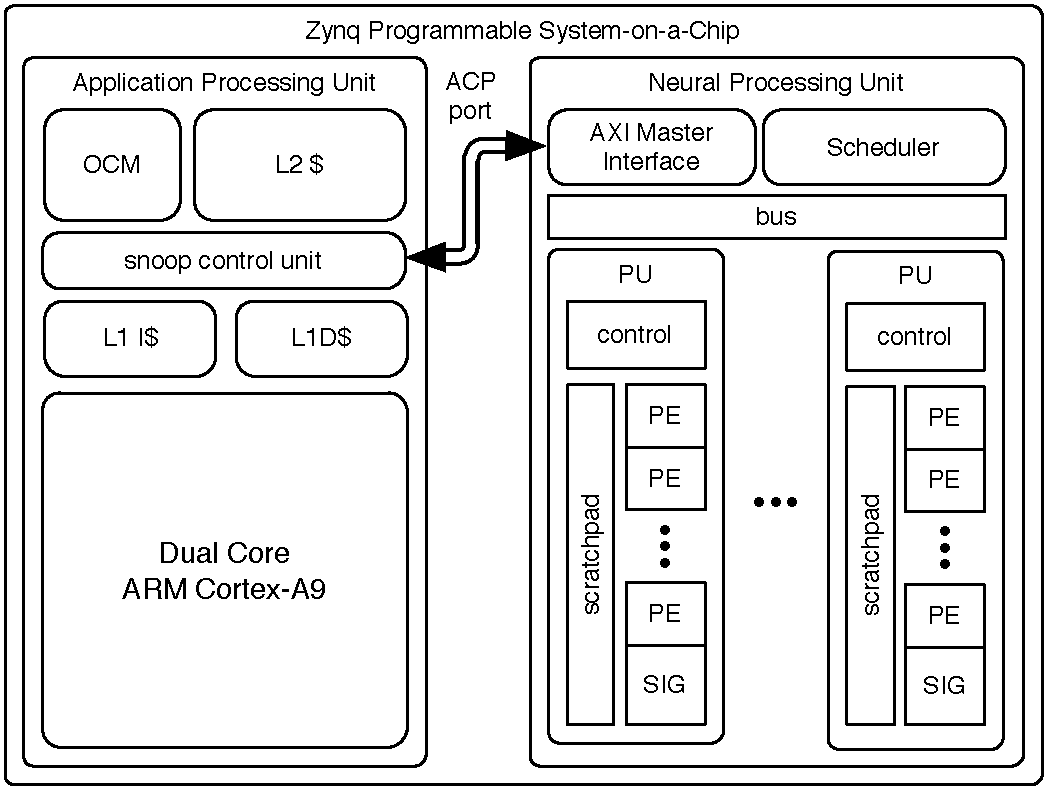
\includegraphics[width=0.8\linewidth]{figs/npu.pdf}
    \vspace{-1.5ex}
    \caption{Neural accelerator system diagram.}
    \label{accept:fig:snnap}
\end{figure}

Our design, shown in  Figure~\ref{accept:fig:snnap}, consists of a cluster of eight processing units (PUs) connected through a bus.
Each PU comprises a control block, a chain of processing elements (PEs),
and a sigmoid unit. The PEs are implemented on DSP logic and form a one-dimensional systolic array that feeds into
the sigmoid unit. When evaluating a neural network layer, PEs read the
synaptic weights from a scratchpad memory.
The sigmoid unit implements a nonlinear neuron-activation function
using a lookup table. At the core of the PU control block lies a configurable sequencer that
orchestrates communication between the PEs and the sigmoid unit. Different
PUs can be individually programmed to evaluate either a single or multiple different neural networks.

% 
% In its simplest form, the NPU is configured
% to accelerate the same neural network schedule across all eight PUs.
% 
% In this case, in order to orchestrate the parallel evaluation
% of neural networks, the NPU scheduler offloads the inputs to each PU in a round-robin fashion.

% Our FPGA-based NPU implementation has direct access to the snoop-control unit of the host processor through the
% accelerator coherency port (ACP). We designed a lightweight AXI master interface on the FPGA to read and write data to the
% processor's caches and on-chip memory (OCM). 

The NPU communicates with
the host processor through the accelerator coherency
port (ACP), which reads and writes data to the
processor's caches and on-chip memory (OCM). The host processor sends the neural network input sets to a region of the OCM that serves as a buffer. 
The host processor then signals the FPGA that the data is ready to be read using
the dedicated event-signaling instructions in
the ARMv7 ISA and transitions to a low-power state until it is awoken by the FPGA.
The FPGA reads the inputs
and evaluates the neural network. As results are generated, they are written back to the OCM, and once the NPU on the FPGA is
done processing the batch, it signals the host CPU that the output is ready. 

Full details on the FPGA design are out of the scope of this paper, since our
focus is on the programming framework, but will be made available in a technical
report after publication.
\fi


\section{Implementation}
\label{passert:sec:implementation}

We implemented \tool using the LLVM compiler infrastructure~\cite{llvm}. \tool
compiles source programs written in C and C++ to the LLVM intermediate
language, probabilistically evaluates the resulting bitcode programs by extracting
probability distributions, optimizes the resulting distributions, and
then evaluates the \passert distributions either exactly or with sampling.

\paragraph{Language and Interface}

To use the verifier system, the programmer adds a \passert to her program and annotates
certain functions as probability distributions or uses a provided library of
common distributions. Both constructs are implemented as C macros provided by
a \texttt{passert.h} header: \texttt{PASSERT(e)} marks an expression that
\tool will evaluate and \texttt{DISTRIBUTION} marks functions
that should be treated as a symbolic probability distribution.

To invoke \tool, the programmer provides arguments comprising the source
files, command-line
arguments for the program under test, and optional $\alpha$ and $\epsilon$ values
that control confidence and accuracy. \tool reports a confidence interval on
the output probability and the results of the hypothesis test (true, false, or
unverifiable).

\paragraph{Distribution Extraction}

The distribution extraction analysis is implemented as an instrumented
interpreter of LLVM bitcode programs. \tool maintains a symbolic heap and
stack. Each symbolic value is a pointer into an object graph representing a
Bayesian network. Nodes in the graph correspond to the expression tree language of
our formalism: they can be samples, arithmetic operations, comparisons,
constants, or conditionals.

The implementation conserves space by coalescing identical expression trees.
For example, consider the values
$e_1 = \{ s_1 + s_2 \}$ and $e_2 = \{ (s_1 + s_2) + s_3 \}$ consisting of sums of samples.
In a naive implementation of probabilistic evaluation, these would be independent trees
that refer to a global set of samples at their leaves.
Instead, \tool implements $e_2$ as a sum node with two
children, one of which is the node for $e_1$.
In this sense, \tool maintains a global Bayesian network for the
execution in which
values are pointers into the network.

Nodes in the Bayesian network can become unreachable when heap values are
overwritten and as stack frames are popped.
\tool reclaims memory in these cases by reference-counting all nodes in the
Bayesian network.
The root set consists of stack and heap values.
Since Bayesian networks are acyclic, reference counting is sufficient.

When operating on non-probabilistic values (e.g., when evaluating $1 + 2$),
\tool avoids constructing nodes in the Bayesian network and instead maintains
a concrete heap and stack. We use
LLVM's bitcode interpreter~\cite{llvminterp} to perform
the concrete operations.
This process can be viewed as an optimization on Bayesian networks for
operations over point-mass distributions.

\edef\optsdata#1{%
\ifstrequal{#1}{gpswalk-arithIdent}{1914}{}%
\ifstrequal{#1}{gpswalk-clt}{1}{}%
\ifstrequal{#1}{gpswalk-knownDist}{0}{}%
\ifstrequal{#1}{hotspot-arithIdent}{1}{}%
\ifstrequal{#1}{hotspot-clt}{1}{}%
\ifstrequal{#1}{hotspot-knownDist}{24064}{}%
\ifstrequal{#1}{inversek2j-arithIdent}{901}{}%
\ifstrequal{#1}{inversek2j-clt}{1}{}%
\ifstrequal{#1}{inversek2j-knownDist}{200}{}%
\ifstrequal{#1}{kmeans-arithIdent}{2149}{}%
\ifstrequal{#1}{kmeans-clt}{0}{}%
\ifstrequal{#1}{kmeans-knownDist}{300}{}%
\ifstrequal{#1}{salary-abs-arithIdent}{5003}{}%
\ifstrequal{#1}{salary-abs-clt}{1}{}%
\ifstrequal{#1}{salary-abs-knownDist}{1}{}%
\ifstrequal{#1}{salary-arithIdent}{3}{}%
\ifstrequal{#1}{salary-clt}{1}{}%
\ifstrequal{#1}{salary-knownDist}{1}{}%
\ifstrequal{#1}{sobel-arithIdent}{7880}{}%
\ifstrequal{#1}{sobel-clt}{1}{}%
\ifstrequal{#1}{sobel-knownDist}{0}{}%
}


\begin{sidewaystable}
    \centering
    \small
    \begin{tabular}{l
    >{\raggedright\arraybackslash} p{2.7in}
    r r r
    r r r}
        \toprule
        &&\multicolumn{3}{c}{Time (seconds)}
        &\multicolumn{3}{c}{Optimization Counts}
        \\ \cmidrule(lr){3-5} \cmidrule(lr){6-8}
        Program &
        Description and \passert &
        Baseline &
        Analysis &
        Sampling &
        Arith &
        Dist Op &
        CLT
        \\
        \midrule
        \bench{gpswalk} &
Location sensing and velocity calculation \newline
\passert: Velocity is within normal walking speed &
\perfdata{time-gpswalk-dummy-run} &
\perfdata{time-gpswalk-sample-analyze} &
\perfdata{time-gpswalk-sample-run} &
\optsdata{gpswalk-arithIdent} &
\optsdata{gpswalk-knownDist} &
\optsdata{gpswalk-clt}
\\
\addlinespace[0.6ex]
\bench{salary} &
Calculate average of concrete obfuscated salaries \newline
\passert: Obfuscated mean is close to true mean &
\perfdata{time-salary-dummy-run} &
\perfdata{time-salary-sample-analyze} &
\perfdata{time-salary-sample-run} &
\optsdata{salary-arithIdent} &
\optsdata{salary-knownDist} &
\optsdata{salary-clt}
\\
\addlinespace[0.6ex]
\bench{salary-abs} &
\bench{salary} with abstract salaries drawn from a distribution \newline
\passert: As above &
\perfdata{time-salary-abs-dummy-run} &
\perfdata{time-salary-abs-sample-analyze} &
\perfdata{time-salary-abs-sample-run} &
\optsdata{salary-abs-arithIdent} &
\optsdata{salary-abs-knownDist} &
\optsdata{salary-abs-clt}
\\
\addlinespace[0.6ex]
\bench{kmeans} &
Approximate clustering \newline
\passert: Total distance is within threshold &
\perfdata{time-kmeans-dummy-run} &
\perfdata{time-kmeans-sample-analyze} &
\perfdata{time-kmeans-sample-run} &
\optsdata{kmeans-arithIdent} &
\optsdata{kmeans-knownDist} &
\optsdata{kmeans-clt}
\\
\addlinespace[0.6ex]
\bench{sobel} &
Approximate image filter \newline
\passert: Average pixel difference is small &
\perfdata{time-sobel-dummy-run} &
\perfdata{time-sobel-sample-analyze} &
\perfdata{time-sobel-sample-run} &
\optsdata{sobel-arithIdent} &
\optsdata{sobel-knownDist} &
\optsdata{sobel-clt}
\\
\addlinespace[0.6ex]
\bench{hotspot} &
Approximate CMOS thermal simulation \newline
\passert: Temperature error is low &
\perfdata{time-hotspot-dummy-run} &
\perfdata{time-hotspot-sample-analyze} &
\perfdata{time-hotspot-sample-run} &
\optsdata{hotspot-arithIdent} &
\optsdata{hotspot-knownDist} &
\optsdata{hotspot-clt}
\\
\addlinespace[0.6ex]
\bench{inversek2j} &
Approximate robotics control \newline
\passert: Computed angles are close to inputs &
\perfdata{time-inversek2j-dummy-run} &
\perfdata{time-inversek2j-sample-analyze} &
\perfdata{time-inversek2j-sample-run} &
\optsdata{inversek2j-arithIdent} &
\optsdata{inversek2j-knownDist} &
\optsdata{inversek2j-clt}
\\

        \bottomrule
    \end{tabular}
    \caption{
        Programs used in the evaluation.
        The \passert for each application describes a probabilistic
        correctness property.
        The \emph{time} columns indicate the time taken by the baseline
        stress-testing strategy, \tool's analysis, and \tool's sampling step.
        The \emph{optimization counts} reflect the three categories of
        optimizations applied by \tool: arithmetic identities (Arith), operations on
        known closed-form distributions (Dist Op), and the Central Limit
        Theorem optimization (CLT).
    }
    \label{passert:table:apps}
\end{sidewaystable}

\paragraph{Conditionals}

Conditionals appear as branches in LLVM IR.
\tool analyzes conditionals by
symbolically executing both sides of the branch and merging the resulting heap
updates. When the analysis encounters a branch, it finds the immediate post-dominator
(ipdom) in the control-flow graph---intuitively, the join point---and begins by taking
the branch. In this phase, it buffers all heap writes in a (scoped) hash table.
Then, when the ipdom is reached, control returns to the
branch and follows the not-taken direction.
Writes in this phase do not go into the scope for the current conditional:
they propagate to the global heap or, if execution is in a nested outer
conditional, to the enclosing hash table scope.
When the ipdom is reached the second time, the buffered writes are
merged into the outer heap using conditional nodes.

\paragraph{Probabilistic Pointers}

\tool partially supports symbolic pointers for probabilistic array
indexing. Programs can load and store from \code{arr[i]} where \code{i} is
probabilistic, which \tool handles with a probabilistic extension of the
theory of
arrays. Pointers and array indices must be finite discrete
distributions so we can enumerate the set of locations to which a pointer $p$
might refer, i.e., those addresses where $p$'s distribution has non-zero
probability.
Loading from a symbolic pointer $p$ yields a distribution that
reflects the set of values at each such location, while storing to
$p$ updates each location to compose its old and new value
under a conditional distribution.

\paragraph{Bayesian Network Optimizations}

\tool performs statistical optimizations as transformations on the Bayesian
network representation as outlined in Section~\ref{passert:sec:optim}. The
optimizations we implemented fall into three broad categories,
which we characterize empirically in the next section.

The first category consists of arithmetic identities, including
binary operators on constants, comparisons with extremes (e.g.,
C's \code{FLT_MAX}), and addition or multiplication with a constant zero.
These optimizations do not exploit the probabilistic properties of the
Bayesian network but compose with more sophisticated optimizations and enhance
the tool's partial-evaluation effect.
The next category consists of operations on known probability distributions,
including the addition of two normal distributions, addition or
multiplication with a scalar, comparison between distributions with disjoint
support, comparison between two uniform distributions, and comparison with a
scalar (i.e., CDF queries).
These optimizations exploit our probabilistic view of the program to apply
well-known statistical properties of common distributions.
The final optimization we evaluate is the Central Limit Theorem, which
collapses a summation of distributions into a single normal.

Some optimizations, such as basic arithmetic identities, are performed
opportunistically on-the-fly during analysis to reduce \tool's memory
footprint.
Others, such as the Central Limit Theorem transformation, operate only on the
complete graph.
Internally, the on-line optimizer also collapses deep trees of commutative
arithmetic operators into ``fat'' sum and product nodes with many children.
This rewriting helps the optimizer identify constants that can be coalesced and
inverse nodes that cancel each other out.



\paragraph{Verification}
As described in Section~\ref{passert:sec:verification}, the prior
optimizations often produce Bayesian networks that \tool can
directly evaluate.  In other cases, \tool must sample the
optimized Bayesian network, in which case \tool generates LLVM bitcode
that samples from the Bayesian network.
The tool then compiles the generated program to machine code and executes
it repeatedly to perform statistical verification.


%%%%%%%%%%%%%%%%%%%%%%%%%%%%%%%%%%%%%%%%%%%%%%%%%%%%%%%%%%%%%%%%%%%%%%%%

\section{Evaluation}
\label{passert:sec:evaluation}


This section describes our experience expressing \passerts in a variety of
probabilistic programs and using \tool to verify them.

\subsection{Benchmarks}

We evaluate \passerts in five probabilistic programs
from three domains: sensors, differential privacy, and approximate
computing. 
Table~\ref{passert:table:apps} summarizes the set of programs and the \passert
statements we added to each.

Programs that compute with noisy sensor data, such as GPS,
accelerometers, and video game motion sensors, behave
probabilistically~\cite{PPT:05,uncertaint}. To demonstrate our
approach on this class of applications, we implemented a common
mobile-phone application: estimating walking speed~\cite{uncertaint}.
\bench{gpswalk} processes a series of noisy coordinate readings from a mobile
phone and computes the walking speed after each reading.
The GPS error follows a Rayleigh distribution and is determined by the sensor's
uncertainty estimate.
As Bornholt et al.~\cite{uncertaint} note, this kind of sensing workload can
produce wild results when an individual location reading is wrong.
The \passert checks that the computed velocity is below a maximum walking
speed.

Differential privacy obfuscates personal data at the cost of
accuracy~\cite{pinq, airavat, gupt, fuzz, certipriv}.
To study how \tool works on this class of application, we
implemented two benchmarks.
\bench{salary} reads a list of 5000 salaries of Washington state public
employees
and computes their average.\footnote{Source: \url{http://fiscal.wa.gov/}}
The program obfuscates each salary by adding a normal distribution ($\sigma^2
= 3000$) to simulate a situation where each employee is unwilling to divulge
his or her exact salary. The \passert checks whether the obfuscated average is
within 25 dollars of the true average.
We also evaluate a version of the program, \bench{salary-abs}, where the input
salaries are drawn from a uniform distribution instead of read from a file.
This variant highlights a scenario where specific inputs are unavailable and
we instead want to check a \passert given an input probability distribution.

The final class of applications is drawn from prior work on
approximate computing: \bench{kmeans}, \bench{sobel}, \bench{hotspot}, and
\bench{inversek2j} represent programs
running on approximate hardware~\cite{truffle, pcmos, stochasticproc}.
\bench{sobel} implements the Sobel filter, an image convolution used in edge
detection.
\bench{kmeans} is a clustering algorithm.
\bench{hotspot} simulates thermal activity on a microprocessor. \bench{inversek2j} uses inverse kinematics to compute a robotic arm's
joint angles given a target position.
Both \bench{kmeans} and \bench{hotspot} are drawn from the Rodinia 2.4
benchmark suite~\cite{rodinia} while \bench{sobel} and \bench{inversek2j} are
approximate applications from Esmaeilzadeh et al.~\cite{npu}.
In all cases, we add random calls that
simulate approximate arithmetic operations on inner computations.
The \passert bounds the error of the program's overall output.
For most benchmarks, the error is measured with respect to the output of a
precise version of the computation, but in \bench{inversek2j}, we use the
corresponding forward kinematics algorithm to check the result.

For both approximate and data privacy programs, we compare a
precise version of a function's output with a perturbed version.
In the sensing workload, \bench{gpswalk}, the data is intrinsically noisy, so
there is no ``ground truth'' to compare against.
For the
purposes of this evaluation, we manually extended the programs to compute both
results. A simple ``desugaring'' step could help perform this transformation
automatically by duplicating the code, removing randomization from one
copy, and returning both results.

\subsection{Performance}

To evaluate \tool's performance benefits,
we compare its total running time against
using a simple stress testing baseline.
The baseline checker adds a \code{for} loop around the entire
probabilistic program and counts the number of times the \passert expression
is true.
The time taken for a \tool verification includes the time to extract and
optimize a probability distribution and to repeatedly sample the
result.
We test all programs with a confidence of $\alpha = 0.05$ and an
accuracy of $\epsilon = 0.01$, which leads to 74147 samples.
(Recall from Section~\ref{passert:sec:sample} that the sample count depends only on the
$\alpha$ and $\epsilon$ parameters and 
 so we sample all programs the
same number of times.)
Table~\ref{passert:table:apps} lists the absolute running times and
Figure~\ref{passert:fig:performance} visualizes the normalized performance.
The timings are averaged over 5 executions collected on a dual-core 2~GHz
Intel Core 2 Duo with 4~GB of memory.
On average, \tool verification takes \perfdata{o-normtime-harmmean-sample} as
long as the strawman checker, for a speedup of
\perfdata{o-speedup-harmmean-sample}.


\begin{figure}
    \centering
    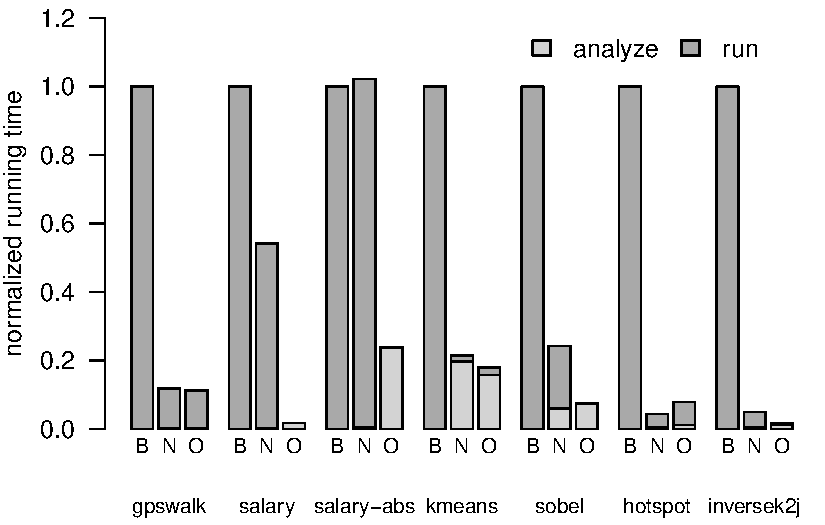
\includegraphics[width=9.5cm]{results/performance}
    \vspace{-1ex}
    \caption{\tool reduces testing time.  We normalize to B: the baseline
      stress-testing technique with 74147 samples. N is \tool without 
      optimizations and O is \tool with optimizations, divided into
      analysis and execution time. Times are averaged over 5 executions.
      We elide error bars as they are very small.}
    \label{passert:fig:performance}
\end{figure}

For most benchmarks, \tool's time is almost exclusively spent on distribution
extraction and optimization, which means optimizations are effective at
producing a very small distribution that can be sampled much more efficiently
than the original program.
The exception is \bench{gpswalk}, where the analysis executed in
\perfdata{time-gpswalk-sample-analyze} seconds
but sampling the resulting distribution took over a minute.
That program's probability distribution consists of thousands of independent
Rayleigh distributions, each with a different parameter as reported by the GPS
sensor, so it cannot take advantage of optimizations that exploit many
samples from identical distributions.

\paragraph{Effect of Optimizations}
We evaluated a variant of \tool with optimizations disabled. This
version simply performs distribution extraction and samples the
resulting distribution.  The middle bars labeled N in
Figure~\ref{passert:fig:performance} show the normalized running time of this
non-optimizing \tool variant.

The effectiveness of the optimizations varies among the benchmarks.
On one extreme, optimizations
reduce the execution time for \bench{salary} from
\perfdata{time-salary-noopt-run} seconds to a fraction of a second.
The unoptimized Bayesian network for \bench{salary-abs} is slightly
\emph{less} efficient than the original program.  The Central Limit
Theorem optimization applies to both and greatly reduces the amount of
sampled computation.  On the other hand, simply evaluating the
extracted distribution delivers a benefit for \bench{gpswalk},
reducing \perfdata{time-gpswalk-dummy-run} to
\perfdata{time-gpswalk-noopt-run} seconds and then optimizations
further reduce this time to just \perfdata{time-gpswalk-sample-run}
seconds.
In a more extreme case, enabling optimizations adds to the analysis time for
\bench{hotspot} but fails to reduce its sampling time.
These programs benefit from eliminating the deterministic
computations involved in timestamp parsing and distance calculation.

\paragraph{Confidence--Performance Trade-off}

Via the confidence and accuracy parameters $\alpha$ and $\epsilon$, \tool
provides rough estimates quickly or more accurate evaluations
using more samples.
% When using fewer samples, the benefits of optimization can be outweighed by
% their costs and the programmer is better off with a brute-force stress-testing
% approach.
To evaluate this trade-off, we lowered the
parameter settings, $\alpha = 0.10$ and $\epsilon = 0.05$, which leads to 2457
samples (about 3\% compared to the more accurate settings above).
Even accounting for analysis time, \tool yields a harmonic mean
\perfdata{o-speedup-harmmean-lowc}
speedup over the baseline in this relaxed configuration.


Approximate computing research combines insights from hardware engineering,
architecture, system design, programming languages, and even application
domains like machine learning. I have confined this section to describe work
that considers the possibility of exposing errors, incorrectness, and
uncertainty to applications. I will not discuss the large body of work on
traditional fault tolerance, which attempts to recover from faults to compute
results without error.

\section{Application-Level Error Tolerance}
\label{sec:related:studies}

Many authors have identified the property of error tolerance in existing
``soft''
applications. A large class of studies have examined this property by
injecting errors into certain parts of applications and assessing the
execution quality in terms of both crashes and output fidelity~\cite{li06,
li07, li08, dekruijf-selse09, wong-selse06, palem-arcs, freton, besteffort,
yeh, thaker-iiswc06, efc, llfi, chippa-dac}.

It is a consensus among many of these studies that different parts of the
application have different impacts on reliability and fidelity. Some conclude
that there is a useful distinction between critical and non-critical program
points (typically instructions)~\cite{palem-arcs, thaker-iiswc06, flikker,
llfi}.
The work tends to assume that at least the instructions involved in control
flow are critical~\cite{thaker-iiswc06}. In my work, I use this idea of
distinguishing between critical and noncritical components to help the
programmer express approximations with bounded effects on the program as a
whole. In each of the approximate system components I have designed, the
execution substrate supports precise (traditional) and relaxed operation to
exploit this distinction. An important question, however, is the granularity
at which to switch between these two modes. \secref{princ:granularity} discusses
this challenge in more detail.

This class of work also typically attempts to classify the kinds of programs
that can tolerate error injection gracefully. For example, papers have focused
on video~\cite{freton}, recognition and mining~\cite{besteffort}, physical
simulation~\cite{yeh}, and optimization~\cite{hogwild}.

Aside from existing software, some studies have evaluated error-resilience in
integrated circuit designs~\cite{breuer, scalable-effort-hardware}. These
studies focus on the kinds of applications that are typically implemented with
application-specific circuits: media codecs, numerical kernels, and digital
signal processing.

Much of the work on application robustness tends to assume an existing,
domain-specific notion of ``quality'' for each
application.
As the principle in \secref{princ:appspecific} suggests, these quality metrics
need careful consideration: one quality metric is not necessarily just as good
as another.
Recent work has proposed guidelines for measuring quality
rigorously~\cite{wddd-quality}.


\section{Exploiting Resilience in Architecture}

The existence of a large class of error-resilient applications has motivated
research into techniques that exploit this property to reduce resource usage.
Specifically, designs have emerged that extend circuits and processor
architectures to trade off error for energy, time, manufacturing yield, or
verification complexity.

Since floating-point operations are both expensive and inexact, they make a
profitable target for this research direction. Researchers have designed units
that dynamically adapt mantissa width~\cite{bitwidthred, hierarchfpu}, ``fuzzily'' memoize
similar arithmetic computations~\cite{fuzzymemo}, or tolerate timing
errors~\cite{kumarhpca, hizli}.
Alternative number
representations work in tandem with relaxed functional units to bound the
numerical error that can result from bit flips~\cite{stanleymarbell}.

The VLSI community has paid particular attention to variable-accuracy adder
designs, which are allowed to yield incorrect results for some minority of
input combinations~\cite{uva-adder, palem-adders, impact, adder-metrics,
configurable-adder, adder-iccad13, adder-tcad, adder-optimal, adder-dac12,
adder-isic09, adder-date08}.

SRAM
structures spend significant static power on retaining data, so they represent
another opportunity for fidelity trade-offs~\cite{hybrid-sram, sramerrors,
partially-forgetful}. Similarly,
DRAM structures can reduce the power spent on refresh cycles where bit flips
are allowed~\cite{flikker, sparkk}.
In persistent memories where storage cells can wear out, approximate systems
can reduce the number of bits they flip to lengthen the useful device
lifetime~\cite{fang-pcm}.
Similarly, low-power writes to memories like flash can exploit its
probabilistic properties while hiding them from software~\cite{halfwits,
powerfade, flash-retention-relax}.
Spintronic memories exhibit similarly favorable trade-offs between access cost
and error~\cite{spintronic-approx}.

Some recent work has also proposed general techniques for making quality trade-offs
when synthesizing and optimizing general hardware
circuits~\cite{lossysynthesis, palem-pruning, rahimi, axilog, miao-thesis}.

As a dual to adding errors in some circuits, some researchers have
explored differential fault protection in the face of universally unreliable
circuits. As process sizes continue to shrink, it is likely that reliable
transistors will become the minority; redundancy and checking will be
necessary to provide reliable operation~\cite{li-asplos08}. Circuit design
techniques have been proposed that reduce the cost of redundancy by providing
it selectively for certain instructions in a CPU~\cite{wreft} or certain
blocks in a DSP~\cite{unequal-protection, ant, micropower-dsp}.
Researchers at Wisconsin have applied relaxed error tolerance at the
architecture level to GPUs~\cite{palframan-gpu}.
Other work has used criticality information to selectively allocate
software-level error detection and correction
resources~\cite{khudia-tolerance, shi-cal}.

Aside from designing fundamentally approximate circuits, a different direction
introduces approximation by relaxing traditional microarchitectural
mechanisms.
Notably, ``soft coherence'' relaxes intercore
communication~\cite{softcoherence},
and load value approximation~\cite{lva-sanmiguel, lva-thwaites} approximates
numerical values instead of fetching them from main memory on cache misses.

Recent work has proposed system organizations that apply approximation at a
coarser grain.
Yetim et al., for instance,
describe a technique that uses coarse-grained quality techniques to
allow errors even in processor control logic~\cite{martonosi-date, commguard}.
Duwe~\cite{duwe-thesis} proposes run-time coalescing of approximate and
precise computations to reduce the overhead of switching between modes.
Other work allocates approximation among the lanes of a SIMD
unit~\cite{tabsh}.

Near-threshold voltage domains also present a new opportunity for embracing
unpredictable circuit operation~\cite{soft-ntc}.

Much of this work on hardware-level approximation work by exposing
soft errors and other analog effects.
Recent work in security and privacy has exploited these variability-related
errors to fingerprint hardware and deanonymize users~\cite{deanondram}.




\section{Exploiting Resilience with Program Transformations}
\label{sec:related:software}

Aside from system-level accuracy trade-offs, there are opportunities for
adapting \emph{algorithms} to execute with varying precision. Algorithmic
quality--complexity trade-offs are not new: approximation algorithms are a
well-studied area of complexity theory and many domains, notably real-time
vision and graphics, have ad-hoc ``cheap'' implementations of computations
that are prohibitively expensive to compute exactly.

In contrast to these
traditional views on approximation, recent work has sought to provide
tools for transforming real programs---as opposed to high-level
algorithmic specifications---to explore practical relaxations.
Transformations include removing portions of a program's dynamic execution
(termed \emph{code perforation})~\cite{perforation}, unsound
parallelization of serial programs~\cite{quickstep}, eliminating
synchronization in parallel programs~\cite{dubstep, races-ibm, hogwild},
identifying and adjusting parameters that control output
quality~\cite{dynamicknobs}, randomizing portions of deterministic
programs~\cite{zhu-popl12, sasa-sas11}, dynamically choosing between
different programmer-provided implementations of the same
specification~\cite{green, virus, petabricks, taco-soc, ansel-autotuning,
scalable-classifier}, and replacing pure computations with invocations
of a trained neural network~\cite{benchnn, temam-isca, emeuro}.

Central to each of these program transformation techniques are the questions
of automation and quality. For a relaxation to be generally useful, it should
be applicable automatically with only minimal programmer involvement but
should still result in transformed code that the programmer is happy with.
Recently, a set of techniques has been proposed to help constrain the space
of possible transformations to those that result in a profitable
quality trade-off. Quality of service profiling~\cite{qosprof} uses many
executions to identify parts of a program that are likely to be good
candidates for transformation. Some verification tools and proof systems help
the programmer prove relationships between the original program and a
candidate relaxed version~\cite{carbin-pldi, carbin-races, carbin-pepm,
rice-transformation-semantics}.
Another approach constrains the programming model to help express programs
that refine their results as they run longer, permitting quality trade-offs in
hard real-time settings~\cite{chung90}.

Recent work from Michigan combines pattern-matching code transformations with
dynamic monitoring to provide approximation trade-offs for GPU
workloads~\cite{paraprox, sage}.
Similarly, Sartori and Kumar~\cite{herding} propose to transform GPU programs
to reduce their control divergence at the cost of correctness.

Recently, a research direction has developed in \emph{automated program
repair} and other approaches to heuristically patching software according to
programmer-specified criteria.
These techniques are typically approximate in that they abandon a traditional
compiler's goal of perfectly preserving the original program's semantics.
Notably, Schulte et~al.~\cite{schulte} propose to use program evolution to
optimize for energy.

Precimonious~\cite{precimonious} addresses the problem of choosing appropriate
floating-point widths, which amount to a trade-off between numerical accuracy
and space or operation cost.
Similarly, STOKE's floating-point extension~\cite{stoke-fp} synthesizes new
versions of floating-point functions from scratch to meet different accuracy
requirements with optimal efficiency.

Neural acceleration is a recent technique treading code as a black box and
transforming it to a neural-network representation.
It is, at its core, an algorithmic transformation, but it integrates tightly
with hardware support: a digital accelerator~\cite{npu}, analog
circuits~\cite{anpu}, FPGAs~\cite{snnap},
GPUs~\cite{neuralgpu}, or, recently, new analog substrates using
resistive memory~\cite{rram-npu} or memristors~\cite{memristor-npu}.
See \secref{npu} for a more detailed overview of neural acceleration.


\section{Dynamically Controlling Approximation}

As an alternative to statically bounding errors, dynamic techniques can
monitor quality degradation at run time.
The critical challenge for these techniques is balancing detection accuracy
with the added cost, which takes away from the efficiency advantages of
approximation.
Some work has suggested that programmers can provide domain-specific checks on
output quality~\cite{lwc, approxdebug}.
Recent work has explored automatic generation of error detectors~\cite{rumba}.
A variety of techniques propose mechanisms for run-time or profiling feedback to adapt
approximation parameters~\cite{dynamicknobs, green, approxit, ansel-autotuning}.
\TODO{describe these in a little more detail}

\section{Languages for Expressing Approximation}

Recently, language constructs that express and constrain
approximation have become a focus in the programming-languages research
community.
Relax~\cite{relax} is a language with ISA support for tolerating architectural
faults in software.
Rely~\cite{rely} uses specifications that relate the reliability of the input
to an approximate region of code to its outputs.

A related set of recent approximate-programming tools attempt to \emph{adapt}
a program to meet accuracy demands while using as few resources as possible.
Chisel~\cite{chisel} is an extension to Rely that searches for the subset of
operations in a program that can safely be made approximate.
ExpAX~\cite{expax-tr} finds safe-to-approximate operations automatically and
uses a metaheuristic to find which subset of them to actually approximate.

\TODO{cite \cite{energytypes}}

\TODO{cite \cite{eon}}


\section{Exploiting Resilience in Other Systems}

While architecture optimizations and program transformations dominate the
field of proposed exploitations of approximate software, some recent work has
explored the same trade-off in other components of computer systems. Network
communication, with its reliance on imperfect underlying channels, exhibits
opportunities for fidelity trade-offs~\cite{softcast, luo-globecom, apex,
smpmup2006}. Notably, SoftCast~\cite{softcast} transmits images and video by
making the signal magnitude directly proportional to pixel luminance. BlinkDB,
a recent instance research on \emph{approximate query answering},
is a database system that can respond to queries that include a required
accuracy band on their output~\cite{blinkdb}.
Uncertain{\textless}T{\textgreater}~\cite{uncertaint} and Lax~\cite{lax}
propose to expose the approximate, probabilistic behavior of sensors at the
language and API levels.
By eschewing redundancy and
recovery in a fault-tolerant distributed system, researchers at Wisconsin were
able to make quality trade-offs in a supercomputing
setting~\cite{dekruijf-icpp}.


\section{Probabilistic Computation}

Several research projects have proposed radically different models of
computation that, rather than adapting existing software to expose its error
resilience, are based exclusively on probabilistic reasoning. Most
prominently, Probabilistic CMOS~\cite{pcmos, pcmos-cacm, palem-dac-position}
and stochastic processors~\cite{stochasticproc} expose the probabilistic
behavior of transistors as part of their ISA.
Other preliminary efforts from MIT~\cite{batesmit, lyric, mansinghka-circuits} and
Stanford~\cite{ersa} fall into the same category.

\section{Probabilistic Semantics}

Researchers have proposed several languages and tools to
help developers better reason about and describe real-world
probabilistic data, computation, and models~\cite{BBGR13,
  wingate-lightweight, church, chaganty, pfeffersample, pmonad,
  infernet, probdsl,uncertaint}.
The probability monad captures a variable's discrete probability
distribution in functional programs~\cite{pmonad}.
\TODO{this one specific call-out is awkward}

Sankaranarayanan et al.~\cite{sriram-pldi} check assertions in
programs that produce probabilistic models using symbolic execution
and polyhedral volume estimation. The \texttt{estimateProbability} construct
queries the probability of an outcome, which resembles a probabilistic
assertion's
specification of the correct outcome.

Statistical model checking bounds verification error on
problems where state-space explosion makes exact numerical
verification intractable (see Legay and Delahaye's
survey~\cite{legay10}).  Model checking~\cite{Clarke} provides formal guarantees,
usually expressed in temporal logic for finite state
based models, often of hardware. For example, the
PRISM tool performs statistical verification of real-time
systems~\cite{KNP11}. Our work borrows the idea of hypothesis
testing to bound error in verification~\cite{Younes,Younes20061368}
and
relies on efficient sampling to avoid
the need for exhaustive state space exploration.

Similarly, recent work has sought to express
uncertainties in the context of traditional, imperative programming
languages~\cite{uncertaint}. These programming models incorporate algorithmic
probabilities---such as those inherent in sensor readings or machine learning
model parameters---but do not yet address the computational probabilities of
techniques like PCMOS and stochastic processors.

Kozen~\cite{kozen} recognizes the need for semantics for programs
that use randomness during execution.
That work provides two semantics for a simple probabilistic
language---one that models sampling and one that computes on probability
distributions directly---and proves them equivalent.
Similarly, we prove equivalence between sampling an original program and
sampling its extracted Bayesian network representation.
Kozen predates the coinage and popularization of Bayesian networks, so
the semantics in that work are very different from the graphical-model approach
presented here.
Our Bayesian-network representation enables statistical optimizations that
make probabilistic assertion verification efficient.
\TODO{this paragraph has dangling references to the passert paper}

\subsection{Probabilistic Programming Languages}

The field of \emph{probabilistic programming} seeks to enable efficient
construction and querying of statistical models~\cite{BBGR13, wingate-lightweight,
  church, chaganty, pfeffersample, probdsl, koller}.  Experts write
generative models as programs and then inference algorithms answer questions
about the model's parameters. The canonical probabilistic programming example
answers, ``given that the grass is wet, was it due to rain or the sprinkler?''




\section{Robustness Analysis}

As the studies in Section~\ref{sec:related:studies} repeatedly find, error
tolerance varies greatly in existing software, both within and between
programs. Several program analysis approaches have been proposed to evaluate
and enhance error resilience properties. SJava analyzes programs to prove that
errors only temporarily disrupt the execution path of a program~\cite{sjava}.
Program smoothing~\cite{smoothing-cav, smoothing-pldi, smoothing-fse} and
``robustification''~\cite{robustification} both find continuous, mathematical
functions that resemble the input--output behavior of numerical programs.
Auto-tuning approaches can help empirically identify error-resilient
components~\cite{asac}.
Finally, Cong and Gururaj describe a technique for automatically
distinguishing between critical and non-critical instructions for the purpose
of selective fault tolerance~\cite{cong-iccad}.


\section{Discussion}

\sysname differs from the other projects in this dissertation in its focus on a
robust, open-source, end-to-end implementation.
The goal is to demonstrate that a common compiler infrastructure can address
the common concerns for a wide variety of realistic approximation
techniques---in the same way that a classical compiler infrastructure like
LLVM provides all the tools that an intrepid compiler hacker needs to build
new optimizations.
This level of generality required that we solve two common challenges:
balancing programmer insight with automation,
and bridging the gap between fine-grained annotations and coarse-grained
optimizations.

The \sysname source code and documentation is available online at: \\
\url{http://sampa.cs.washington.edu/accept}

